\documentclass{article}
\usepackage[utf8]{inputenc}

\title{An Analysis of Penalized Regression in High Dimensional Scenarios}
\author{Gabriel Ackall$^1$*, Connor Shrader$^2$* \\
	Mentor: Dr. Seongtae Kim$^3$ \\	
	{\footnotesize $^1$Georgia Tech, Civil Engineering} \\
	{\footnotesize $^2$University of Central  Florida, Mathematics} \\
	{\footnotesize $^3$NCA\&T University, Mathematics and Statistics} \\
	{\footnotesize *Authors contributed equally}}
\date{\today}

% Format settings
\setlength{\parskip}{6pt}

% Package imports
\usepackage{fancyhdr}
\usepackage[margin = 1.5in]{geometry}

\usepackage{amsmath}
\usepackage{amsthm}
\usepackage{listings} % Show code in LaTeX
\usepackage{graphicx} % Figures
\usepackage{caption} % Caption customization
\usepackage{subcaption} % Subfigures
\usepackage{url}
\usepackage{adjustbox}
\usepackage{hyperref} % Clickable ref's
\usepackage{lscape}
\usepackage{multirow}
\usepackage{bm}

% Tikz stuff
\usepackage{tikz}
\usetikzlibrary{shapes.geometric, arrows}
\usepackage{forest}

\tikzstyle{fit} = [rectangle, inner sep = 0.2cm, rounded corners, minimum height = 0.6cm, text centered, draw = black, fill = cyan!20]
\tikzstyle{tree} = [rectangle, inner sep = 0.2cm, rounded corners, minimum height = 0.6cm, text centered, draw = black, fill = green!20]

% Caption format
\captionsetup[figure]{font=small}

% Setting up headers and footers
\pagestyle{fancy}
\fancyhead[L]{Penalized Regression}
\fancyhead[R]{Ackall, Shrader}
\fancyfoot[C]{\thepage}

% Set code appearance
\lstset {
	language = R,
	basicstyle = \ttfamily
}

% Clickable link setup
\hypersetup{
	colorlinks=true,
	linkcolor=blue,
	filecolor=magenta,      
	urlcolor=cyan,
	citecolor=blue
}

\newcommand{\argmin}[2]{\underset{#1}{\text{arg min}}\left\{#2\right\}}
\newcommand{\sign}{\text{sign}}
\newcommand{\E}{\text{E}}
\newcommand{\OLS}{\text{OLS}}
\newcommand{\RSS}{\text{RSS}}

\begin{document}
\maketitle
\begin{abstract}
	With the prevalence of big data in recent years, the importance of modeling high dimensional data and selecting influential features has increased greatly. High dimensional data is common in many fields such as genome decoding, rare disease identification, economic modeling, and environmental modeling. However, most traditional regression machine learning models are not designed to handle high dimensional data or conduct variable selection. In this paper, we investigate the use of penalized regression methods such as ridge, least absolute shrinkage and selection operation (lasso), elastic net (E-net), smoothly clipped absolute deviation (SCAD), and minimax concave penalty (MCP) compared to traditional machine learning models such as random forest, XGBoost, and support vector machines. We evaluate these models using factorial design methods for Monte Carlo simulations in 270 environments, with factors being the number of predictors, number of samples, signal to noise ratio, covariance matrix, and correlation strength. We also compare different models using empirical data to evaluate their viability in real-world scenarios. Since our models are regression models, we evaluate the models using the test mean squared error, variable selection accuracy, $\beta$-sensitivity, and $\beta$-specificity. From our investigation, our findings indicate that penalized regression models outperform more traditional machine learning algorithms in most high-dimensional situations or in situations with a low number of data observations. Machine learning models are not often compared to penalized regression methods and so our analysis helps to expand the scope of how penalized regression is used to help model data. Additionally, the analysis helps to create a greater understanding of the strengths and weaknesses of each model type and provide a reference for other researchers on which machine learning techniques they should use, depending on a range of factors and data environments. \\
	
	\textit{Keywords:} penalized regression, variable selection, classification, machine learning, large $p$ small $n$ problem, Monte Carlo simulations
\end{abstract}

\section{Introduction}
% introduce readers to our topic and necessary info to better understand the paper

In the modern world, machine learning techniques such as random forest, gradient boosting, and support vector machines are often touted as versatile one-size-fits-all solutions when it comes to modeling big data \cite{nielsen2016tree}. This is due in part to tree based models such as XGBoost winning numerous machine learning competitions \cite{nielsen2016tree}. While this versatility is frequently the case, an increasingly common type of data set where there are more predictors than observations can pose challenges for these machine learning algorithms. In these situations, lesser known statistical modeling techniques that perform variable selection can potentially perform equivalently or even better than these machine learning techniques. However, there is a distinct lack of academia focusing on comparing these variable selection techniques with the more traditional machine learning techniques. This paper serves to help bridge that gap.

In these situations where there are more predictors, $p$, than observations, $n$, many traditional machine learning techniques either become infeasible to use or fail to give good predictions. The large number of predictors and small number of observations make it easy for such models to \textbf{overfit}, meaning that the models become fine tuned to the exact training data and instead of finding generalized patterns for a population of data, they find specific occurrences in the training data \cite{james2013introduction, friedman2001elements}. Because of this, overfitted models are sensitive to new data which causes them to perform extremely well on the training data, but poorly on testing data or when deployed in the real world. Because a model's predictions in real world scenarios and on new data is the entire purpose of a model, it is very important to reduce overfitting so that predictive accuracy in these scenarios is maximized.

This paper investigates several methods to handle the large $p$, small $n$ problem. First, We considered wrapper methods such as forward selection, backward selection, stepwise forward selection and stepwise backward selection using both Akaike information criterion (AIC) and Bayesian information criterion (BIC) as the stopping criteria for the models \cite{akaike1998information, schwarz1978estimating}. These models fit several linear models using different subsets of predictors and selects the model that optimizes a specific metric. In addition, we studied penalized regression models such as ridge regression \cite{hoerl1970ridge}, least absolute shrinkage and selection operation (lasso) \cite{tibshirani1996regression}, elastic-net \cite{zou2005regularization}, smoothly clipped absolute deviation (SCAD) \cite{fan2001variable}, and minimax concave penalty (MCP) \cite{zhang2010nearly}. These models simultaneously select important predictors and fit a linear model. Finally, we considered a few machine learning models: random forests (RF) \cite{breiman2001random}, gradient boosting in the form of XGBoost \cite{chen2021xgboost}, and support vector machine (SVM) models \cite{cortes1995support}. These models do not assume a linear relationship between a response and its predictors. To compare these different techniques, models were trained and evaluated using both Monte Carlo simulations and empirical genomic data.

Section \ref{sec:methodology} contains details about each model and details the implementation of these models for our study. Section \ref{sec:simulations} describes our simulation study design and results, while section \ref{sec:empirical} explains our empirical data analysis and results. Section \ref{sec:discussion} is a discussion of our results and Section \ref{sec:conclusion} is the conclusion.

\section{Methodology}\label{sec:methodology}
\subsection{Subset Selection Methods}
% We can review some relevant literature such as Tibshrani et. al. lasso methods, ridge regression, enet, SCAD, or whatever else we want to do.

\textbf{Subset selection methods} are wrapper methods that attempt to find a subset of the predictors $X_1, X_2, \dotsc, X_p$ that are most correlated with the response variable $Y$. These algorithms usually fit models for many different subsets and choose the subset of predictors that results in the best model. Although subset selection techniques can be applied to many types of models, we will focus on subset selection with linear regression.

%There are two main benefits to using subset selection methods. By reducing the set of available predictors to just those that are strongly related to the response, overfitting can be mitigated. Another benefit of subset selection is that it creates a more interpretable model. If a data set includes thousands of predictors but only a few are related to the response, a model found using subset selection will be easier to understand than a model that relies on all of the parameters. 

Two subset selection methods we consider are \textbf{forward selection} and \textbf{backward selection}. Forward selection begins by fitting a model with no predictors (only the intercept is non-zero) and iteratively adds predictors into the model. The predictor added at each step is chosen to best increase the model fit. Conversely, backward selection starts from the full (ordinary least squares) model with all $p$ predictors and repeatedly removes predictors. Then, like best subset selection, the final model is chosen from the candidate models fitted at each step. Note that backward selection can only be used when $p\leq n$ since ordinary least squares cannot be used when $p>n$. Forward selection can always be used.

Although forward and backward selection will not always encounter the best possible model, these methods help optimize best subset selection and are quicker than best subset selection. Consequently, forward and backward selection can be used for larger values of $p$. However, despite these optimization, forward and backwards selection are still plagued by the fact that the number of combinations of predictors increases exponentially and thus they cannot be used for very large values of $p$.

The models produced by forward and backward selection can be improved by allowing predictors to be added and removed in the same algorithm. \textbf{Forward stepwise selection} begins with an empty model and iteratively improves the model by either adding a new predictor or removing an obsolete one. \textbf{Backward stepwise selection} works in the same way but starts with the full model. Like backward selection, backward stepwise selection can only be used when $p\geq n$. These techniques take longer to run than ordinary forward and backward selection, but they are more likely to find the best possible model.

When fitting a model using any of the subset selection methods, the performance metric used to select the best model is very important. At first, it may seem reasonable to choose a metric such as the residual sum of squares from Equation \ref{eqn:RSS}. However, many metrics, including the residual sum of squares, only describe a model's performance on training data. This is problematic because including more predictors will always decrease the residual sum of squares on the training data. If $p\leq n$, then the model fitted with all $p$ predictors is exactly the same model produced by ordinary least squares, which by definition minimizes the residual sum of squares! If $p>n$, then a model with the maximum possible number of predictors would be selected.

If we wish to produce a model that makes reliable predictions on test data, we must use a different performance metric. Two of the most common metrics used for this purpose are the \textbf{Akaike information criterion} (AIC) and the \textbf{Bayesian information criterion} (BIC) \cite{akaike1998information, schwarz1978estimating}. For a given model, the Akaike information criterion can be computed by
\begin{equation}
	\text{AIC} = 2p - 2\ln(L)
\end{equation}
where $p$ is the number of predictors for the model and $L$ is the likelihood of the model. This likelihood represents how well a model fits to the training data. The purpose of the term $2p$ is to punish models with a large number of coefficients. The model with the lowest AIC is the one selected by the wrapper methods.

The Bayesian information criterion very similar to the Akaike information criterion; it is given by
\begin{equation}
	\text{BIC} = p\ln(n) - 2\ln(L)
\end{equation}
where again $p$ is the number of predictors for the model and $L$ is the likelihood of the model.

Note that if $n>7$, then $\ln(n)>2$ and so the penalty for BIC is larger than the penalty for AIC. Hence, a model selected using BIC will typically have fewer parameters than a model selected by AIC.

In addition to AIC and BIC, there are several other metrics that modify training error to estimate test error, such as $C_p$ and adjusted $R^2$ \cite{james2013introduction}. However, this paper will focus on AIC and BIC.
\subsection{Penalized Regression}

In general, \textbf{penalized regression} works by fitting a model that punishes large coefficient estimates. By forcing coefficient values to shrink, the resulting model will have relatively low variance. All of the models discussed here can be used when there are more predictors than observations. Most, but not all, of these methods can also perform variable selection.

Almost all of the penalized regression methods in this paper solve an optimization problem of the form
\begin{equation}\label{eqn:penalized-regression-lambda}
	\hat{\bm{\beta}}=\argmin{\bm{\beta}}{\sum\limits_{i = 1}^n \Big[y_i - (\beta_0 + \beta_1 x_{i1} + \beta_2 x_{i2} + \cdots + \beta_p x_{ip})\Big]^2 + \lambda\sum\limits_{j = 1}^p P(\beta_j)}
\end{equation}
where the first summation is the usual residual sum of squares, $\lambda\geq 0$ is a hyperparameter that controls the strength of the penalty, and $P(\beta)$ is a penalty function applied to each of the coefficients. The penalty is not applied to the intercept $\beta_0$. In general, $P(\beta)$ is an even function that is non-decreasing as $\vert \beta \vert$ increases. If $\lambda = 0$, then we have the usual ordinary least squares estimator. As $\lambda$ increases, a stronger penalty is applied which will decrease the coefficient values. As $\lambda$ approaches $\infty$, the model becomes an empty model where only the intercept term is non-zero.

When fitting penalized regression models, the choice of $\lambda$ is very important. If $\lambda$ is too small, then models may be overfit just like ordinary least squares; on the other hand, if $\lambda$ is large, then the resulting models are highly biased and the resulting models may be underfit. In practice, the best value of $\lambda$ can be selected using \textbf{cross validation} and \textbf{grid search}. This process involves splitting the training set into $k$ disjoint subsets of equal size called \textbf{folds}. Then, $k$ models are fitted for different values of $\lambda$, where one fold is used as a testing set and the other $(k - 1)$ folds are used for training. The value of $\lambda$ that results in the lowest test error can then be selected.

\textbf{Ridge regression} is a penalized regression model that uses the penalty function $P(\beta) = \beta^2$ \cite{hoerl1970ridge}. One advantage of ridge regression is that it can handle highly correlated data better than ordinary least squares. When predictors are correlated with each other, some algorithms have a hard time distinguishing which predictors are actually related to the response.

One drawback of ridge regression is that it cannot perform variable selection. It can shrink coefficients towards zero, but it cannot set coefficients to be exactly zero.

The \textbf{least absolute shrinkage and selection operation}, commonly referred to as \textbf{lasso}, is a shrinkage method with a very similar form to ridge regression \cite{tibshirani1996regression, james2013introduction}. The penalty function for lasso is $P(\beta) = \vert \beta \vert$.

Unlike ridge regression, lasso regression can perform variable selection by setting coefficients to zero. This makes lasso regression favorable when most predictors are not related to the response variable. On the other hand, if the response truly does depend on all of the predictors, then lasso regression may incorrectly set some coefficients to zero. In addition, lasso regression does not have a closed-form solution, but computing the coefficients is still efficient.

Figure \ref{fig:ridge-lasso-diagram} provides a visual explanation for why ridge regression cannot perform variable selection while lasso regression can. Suppose that there are $p = 2$ predictors. The red circle in Figure \ref{fig:ridge-diagram} represents the circle $\beta_1^2 + \beta_2^2 \leq t$, which is the penalty boundary for ridge regression when $t = 1$. The red square in Figure \ref{fig:lasso-diagram} represents the boundary $\vert \beta_1 \vert + \vert \beta_2 \vert \leq t$ for lasso regression. The point in the center of the blue ellipses represents the values of $\beta_1$ and $\beta_2$ that ordinary least squares would estimate. Because this point is not within either of the red regions, ridge regression and lasso regression will give different coefficient estimates. The blue ellipses around this point represent contour curves for the residual sum of squares, which is a quadratic function of $\beta_1$ and $\beta_2$. The first intersection of these ellipses with the red regions represents the coefficient values selected by ridge and lasso regression, since it represents the point within the red region with the lowest residual sum of squares. Because the ridge regression boundary is round, the intersection in Figure \ref{fig:ridge-diagram} occurs when $\beta_1$ and $\beta_2$ are both positive. For lasso regression in Figure \ref{fig:lasso-diagram}, the intersection occurs at a corner where $\beta_1=0$. Thus, lasso regression has set $\beta_1$ to zero, while $\beta_1$ is non-zero for ridge regression.

\begin{figure}[!b]
	\centering
	\begin{subfigure}[b]{0.45\textwidth}
		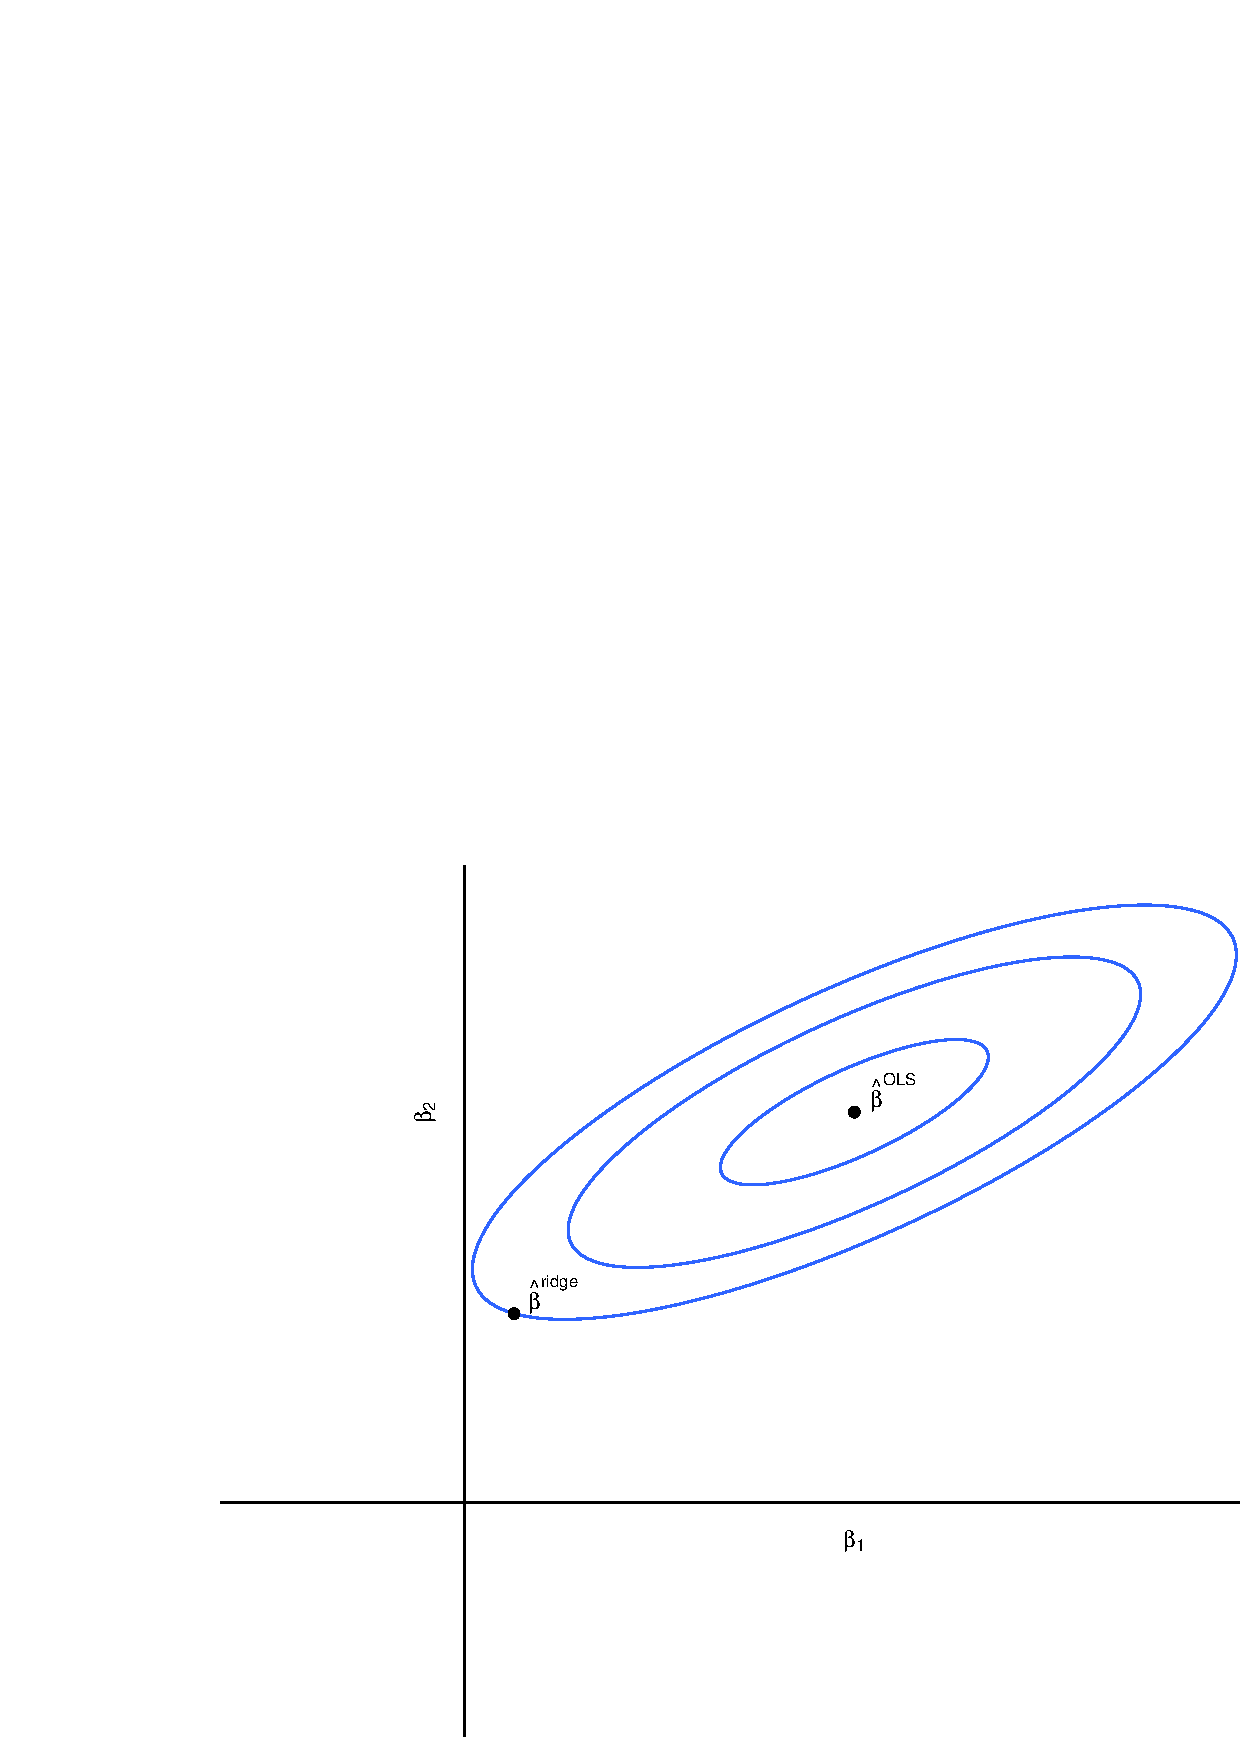
\includegraphics[width=\textwidth]{images/ridge-diagram.png}
		\captionsetup{width = 0.8\textwidth}
		\caption{RSS contours and the ridge penalty boundary.}
		\label{fig:ridge-diagram}
	\end{subfigure}
	\hspace{30pt}
	\begin{subfigure}[b]{0.45\textwidth}
		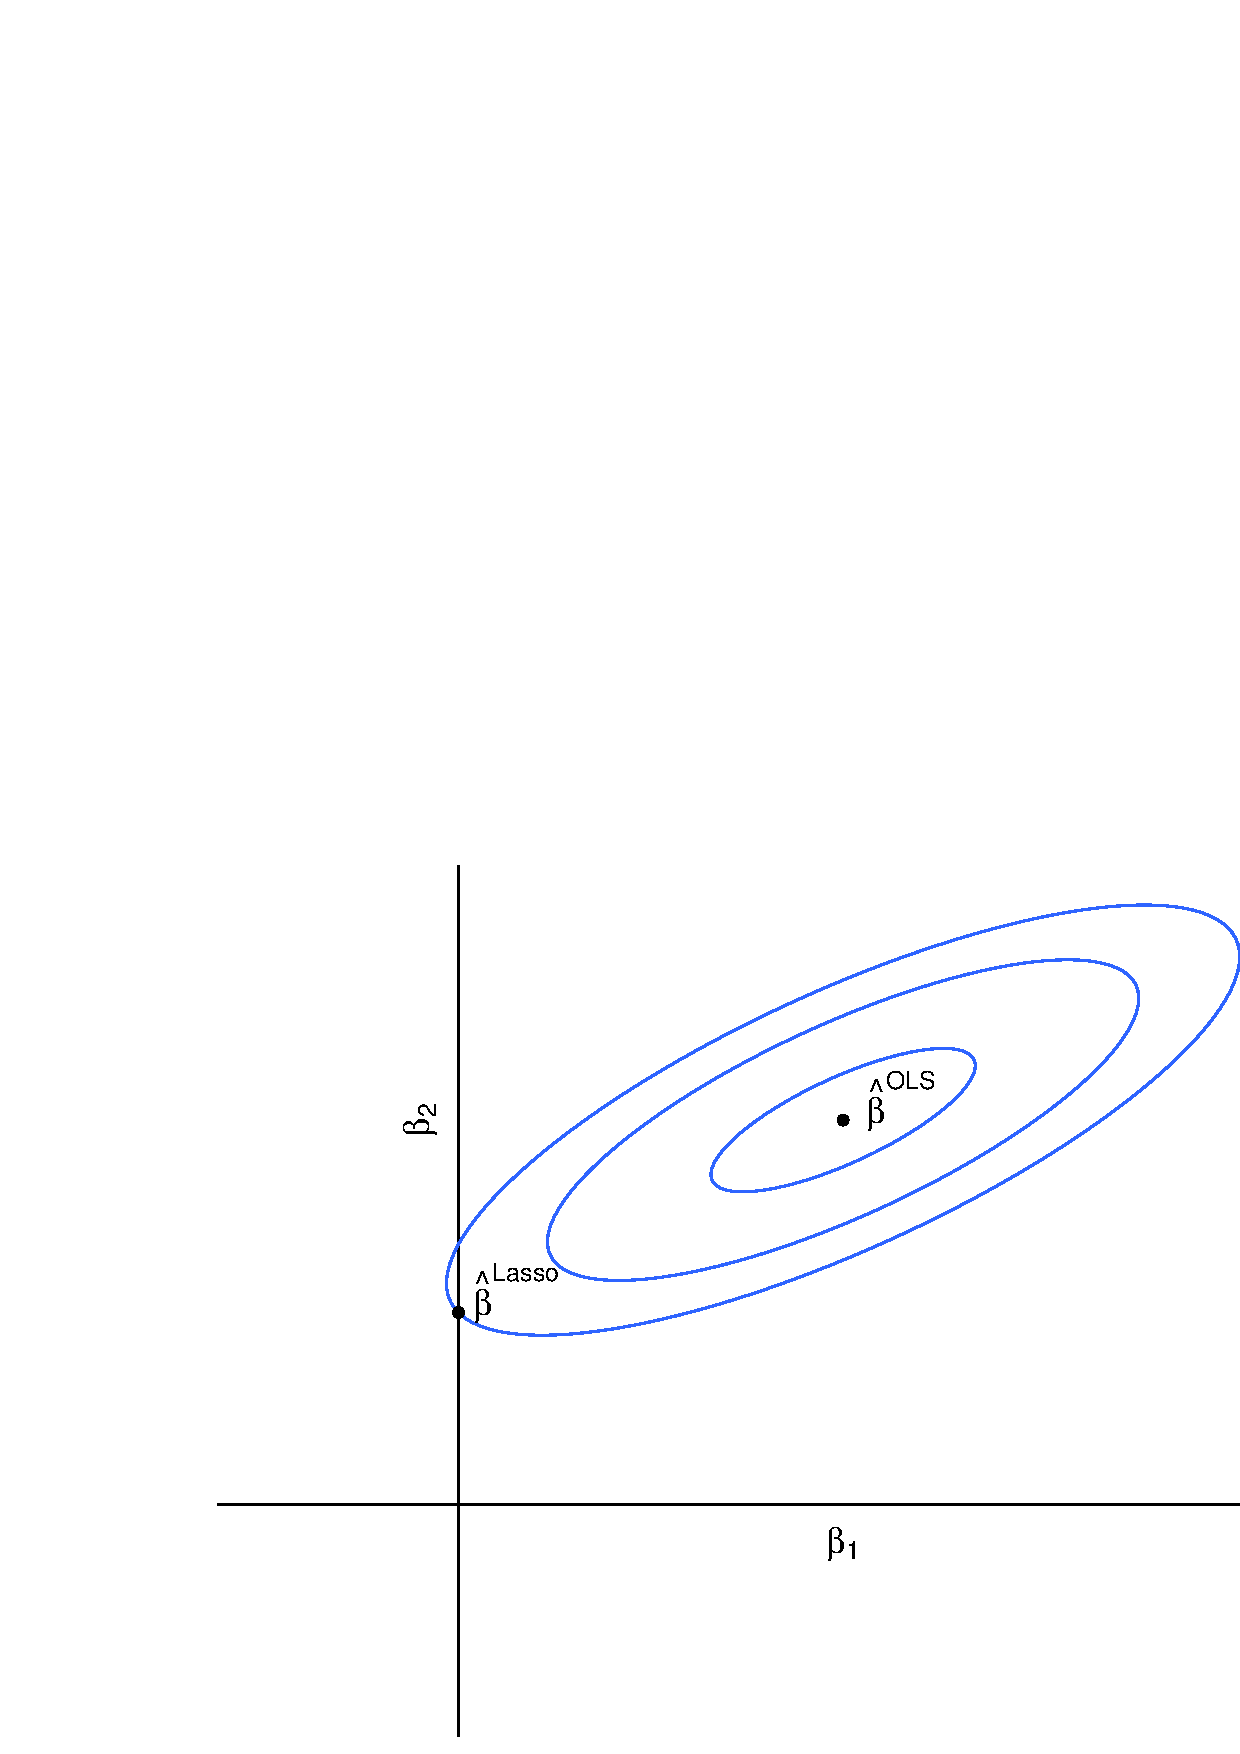
\includegraphics[width=\textwidth]{images/lasso-diagram.png}
		\captionsetup{width = 0.8\textwidth}
		\caption{RSS contours and the lasso penalty boundary.}
		\label{fig:lasso-diagram}
	\end{subfigure}
	\captionsetup{width = 0.9\textwidth}
	\caption{RSS contours and penalty bounds for the ridge and lasso models when $p=2$ and $t = 1$. The red regions represent the coefficient values allowed by ridge and lasso regression, respectively. The blue ellipses represent contours of the residual sum of squares, with $\hat{\beta}^{\text{OLS}}$ being the point where the residual sum of squares is minimized. The intersection of the ellipse with the red region in each plot represents the coefficient values selected by lasso and ridge.}
	\label{fig:ridge-lasso-diagram}
\end{figure}

\textbf{Elastic-net} regression uses both the ridge penalty and the lasso penalty at the same time \cite{zou2005regularization}. Elastic-net solves the optimization problem
\begin{equation}
	\hat{\beta}^{\text{E-net}}=\argmin{\beta}{\sum\limits_{i = 1}^n \Big[y_i - (\beta_0 + \beta_1 x_{i1} + \beta_2 x_{i2} + \cdots + \beta_p x_{ip})\Big]^2 + \lambda_2\sum\limits_{j = 1}^p \beta_j^2 + \lambda_1\sum\limits_{j = 1}^p \vert \beta_j \vert}
\end{equation}
where $\lambda_1$ and $\lambda_2$ are both tuning parameters.

An important limitation to note is that elastic net performs best when it close to either ridge or lasso regression, meaning that either $\lambda_1$ greatly exceeds $\lambda_2$ or $\lambda_2$ greatly exceeds $\lambda_1$ \cite{zou2005regularization}. Additionally, because elastic net requires two tuning parameters, this makes it much more difficult to determine the best combination of tuning parameters to minimize error in the regression. However, this problem has been largely solved through by the LARS-EN algorithm developed by Zou et. al. which efficiently solves for the tuning parameters \cite{zou2005regularization}.

One major flaw of the lasso method is that the penalty punishes large coefficients, even if those coefficients should be large. One way to modify the lasso method is to use the \textbf{smoothly clipped absolute deviation} (SCAD) penalty \cite{fan2001variable}. The goal of this method is to punish large coefficients less severely, which can help mitigate some of the bias introduced by the lasso method. The penalty function $P(\beta)$ for SCAD satisfies
\begin{equation}\label{eqn:scad-derivative-indicator}
	\frac{dP}{d\beta} = \sign(\beta)\left[ I(\vert \beta \vert<\lambda) + \frac{\max(a\lambda - \vert \beta\vert, 0)}{(a - 1)\lambda}I(\vert \beta \vert > \lambda) \right]
\end{equation}
where $a>2$ is a new hyperparameter and $I$ is the indicator function ($I(Q)$ equals 1 if a statement $Q$ is true, and equals 0 if $Q$ is false). If the hyperparameter $a$ is large, then SCAD behaves like lasso for larger coefficient values. Also, notice that $\lambda$ is an argument for the penalty function $P$.

An equivalent way to write the expression in Equation \ref{eqn:scad-derivative-indicator} is
\begin{equation}
	\frac{dP}{d\beta} = \left\{\begin{array}{ll}
		1,&\vert \beta \vert\leq \lambda\\
		\frac{a\lambda - \vert \beta \vert}{(a - 1)\lambda},&\lambda < \vert \beta \vert < a\lambda\\
		0,&\alpha\lambda < \vert \beta \vert
	\end{array}\right.
\end{equation}
This penalty function does not punish coefficients with large magnitude as heavily as the lasso method. In fact, if the magnitude of a coefficient is larger than $a\lambda$, then the penalty becomes constant since the derivative becomes zero.

By integrating with respect to $\beta$ and choosing $P(\beta) = 0$ \cite{breheny2016lasso}, we see that
\begin{equation}
	P(\beta) = \left\{\begin{array}{ll}
		\vert \beta \vert,&\vert \beta \vert \leq \lambda\\
		\frac{2a\lambda\vert\beta\vert - \beta^2-\lambda^2}{2(a - 1)\lambda},&\lambda < \vert \beta \vert \leq a\lambda\\
		\frac{\lambda(a + 1)}{2},&a\lambda < \vert \beta \vert
	\end{array}\right.
\end{equation}

The \textbf{minimax concave penalty} (MCP) method is very similar to SCAD \cite{zhang2010nearly}. Both methods are used to avoid the high bias caused by the lasso method. MCP uses a penalty function that satisfies
\begin{equation}
	\frac{dP}{d\beta} = \left\{\begin{array}{ll}
		\sign(\beta)\left(1 - \frac{\vert \beta \vert}{a\lambda}\right),& \vert \beta \vert \leq a\lambda\\
		0,&a\lambda < \vert \beta \vert
	\end{array}\right.
\end{equation}
where, like SCAD, $a>0$ is a hyperparameter. Integrating \cite{breheny2016lasso}, we see that
\begin{equation}
	P(\beta) = \left\{\begin{array}{ll}
		\vert \beta \vert - \frac{\beta^2}{2a\lambda},&\vert \beta \vert \leq a\lambda\\
		\frac{1}{2}a\lambda,&a\lambda < \vert \beta \vert
	\end{array}\right.
\end{equation}

Figure \ref{fig:lasso-scad-mcp} below shows the penalty functions (and their derivatives) for lasso, SCAD, and MCP as a function of a coefficient value $\beta$. We see that lasso applies a much stronger penalty to large coefficients than SCAD or MCP. Also, note that SCAD starts with a derivative equal to that of the lasso for small values of $\beta$; on the other hand, the derivative of the penalty function for MCP starts decreasing immediately.

\begin{figure}[!h]
	\centering
	\begin{subfigure}[b]{0.45\textwidth}
		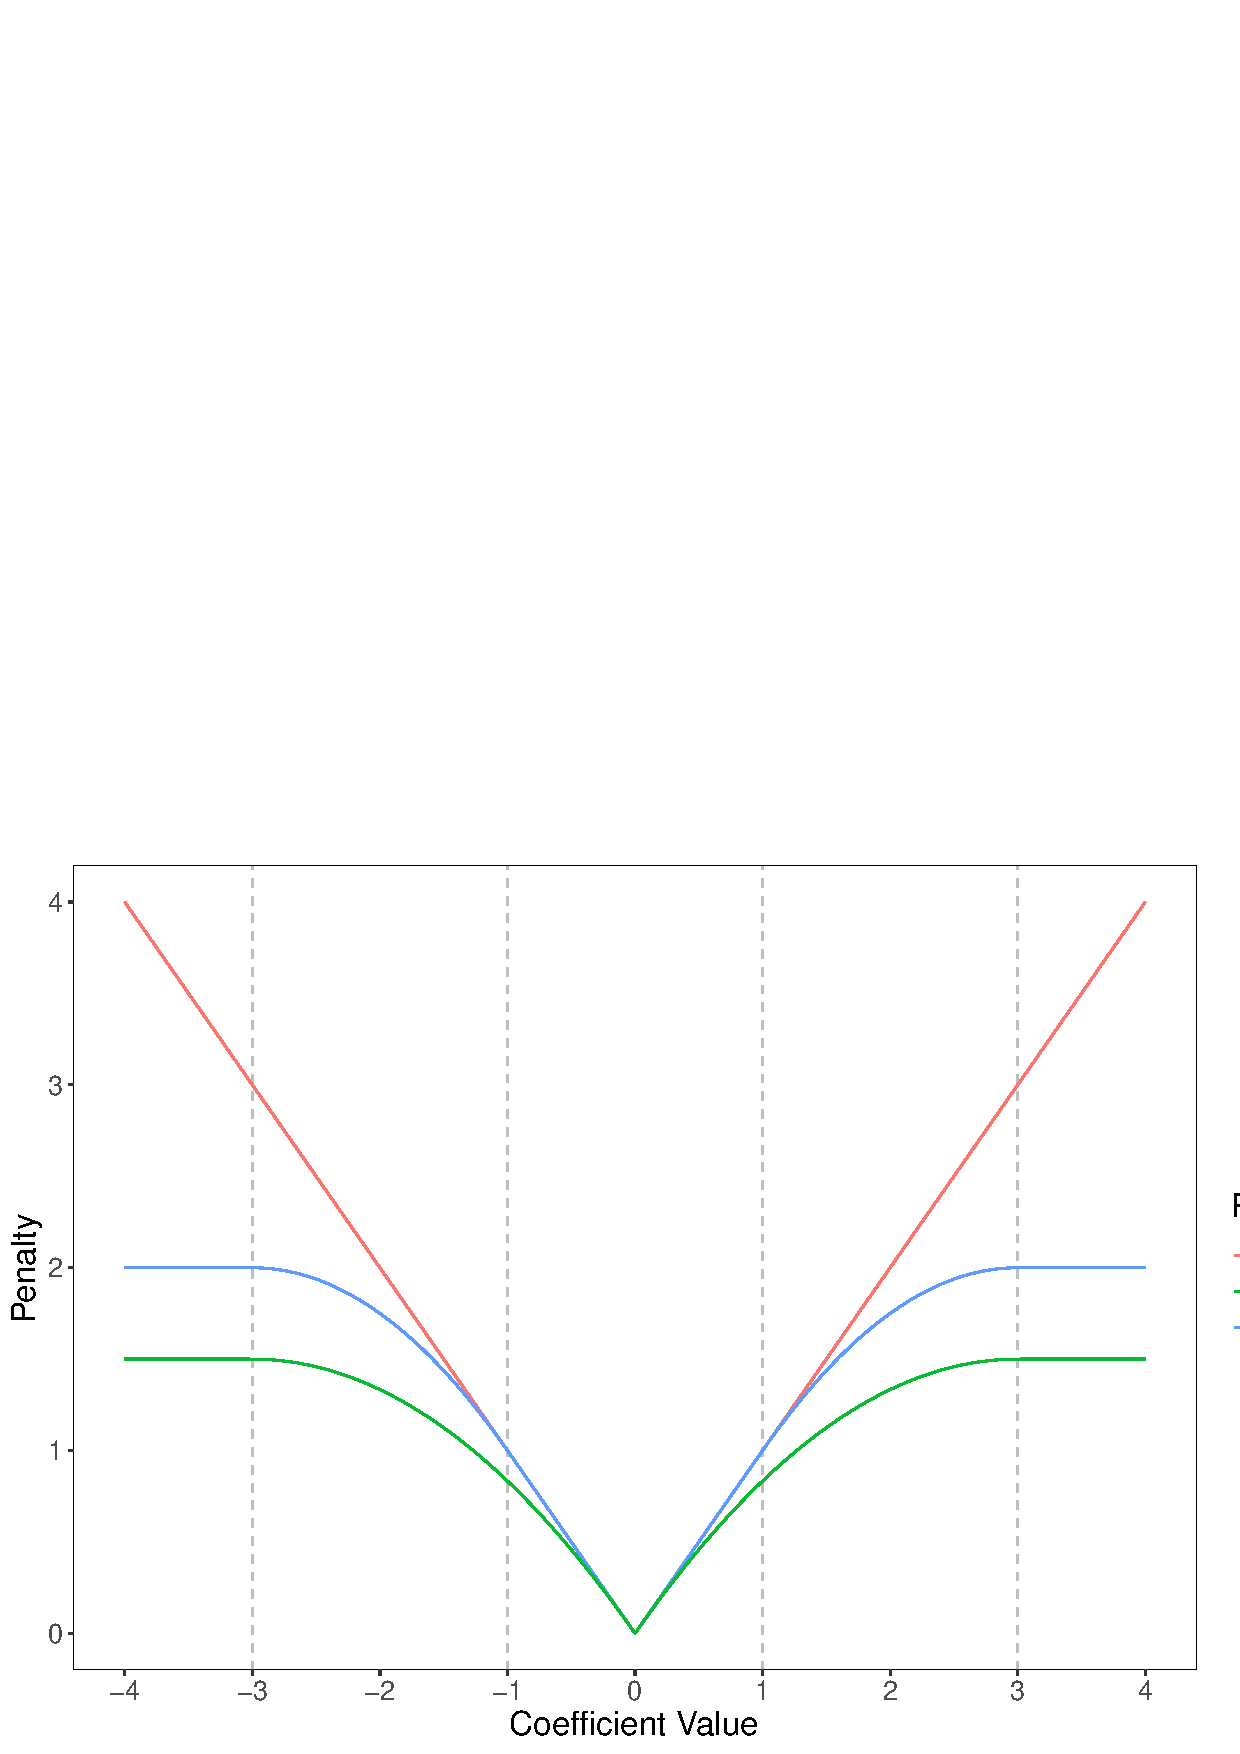
\includegraphics[width=\textwidth]{images/lasso-scad-mcp-penalty.png}
		\captionsetup{width = 0.8\textwidth}
		\caption{Penalty functions for lasso, SCAD, and MCP.}
		\label{fig:penalty}
	\end{subfigure}
	\hspace{30pt}
	\begin{subfigure}[b]{0.45\textwidth}
		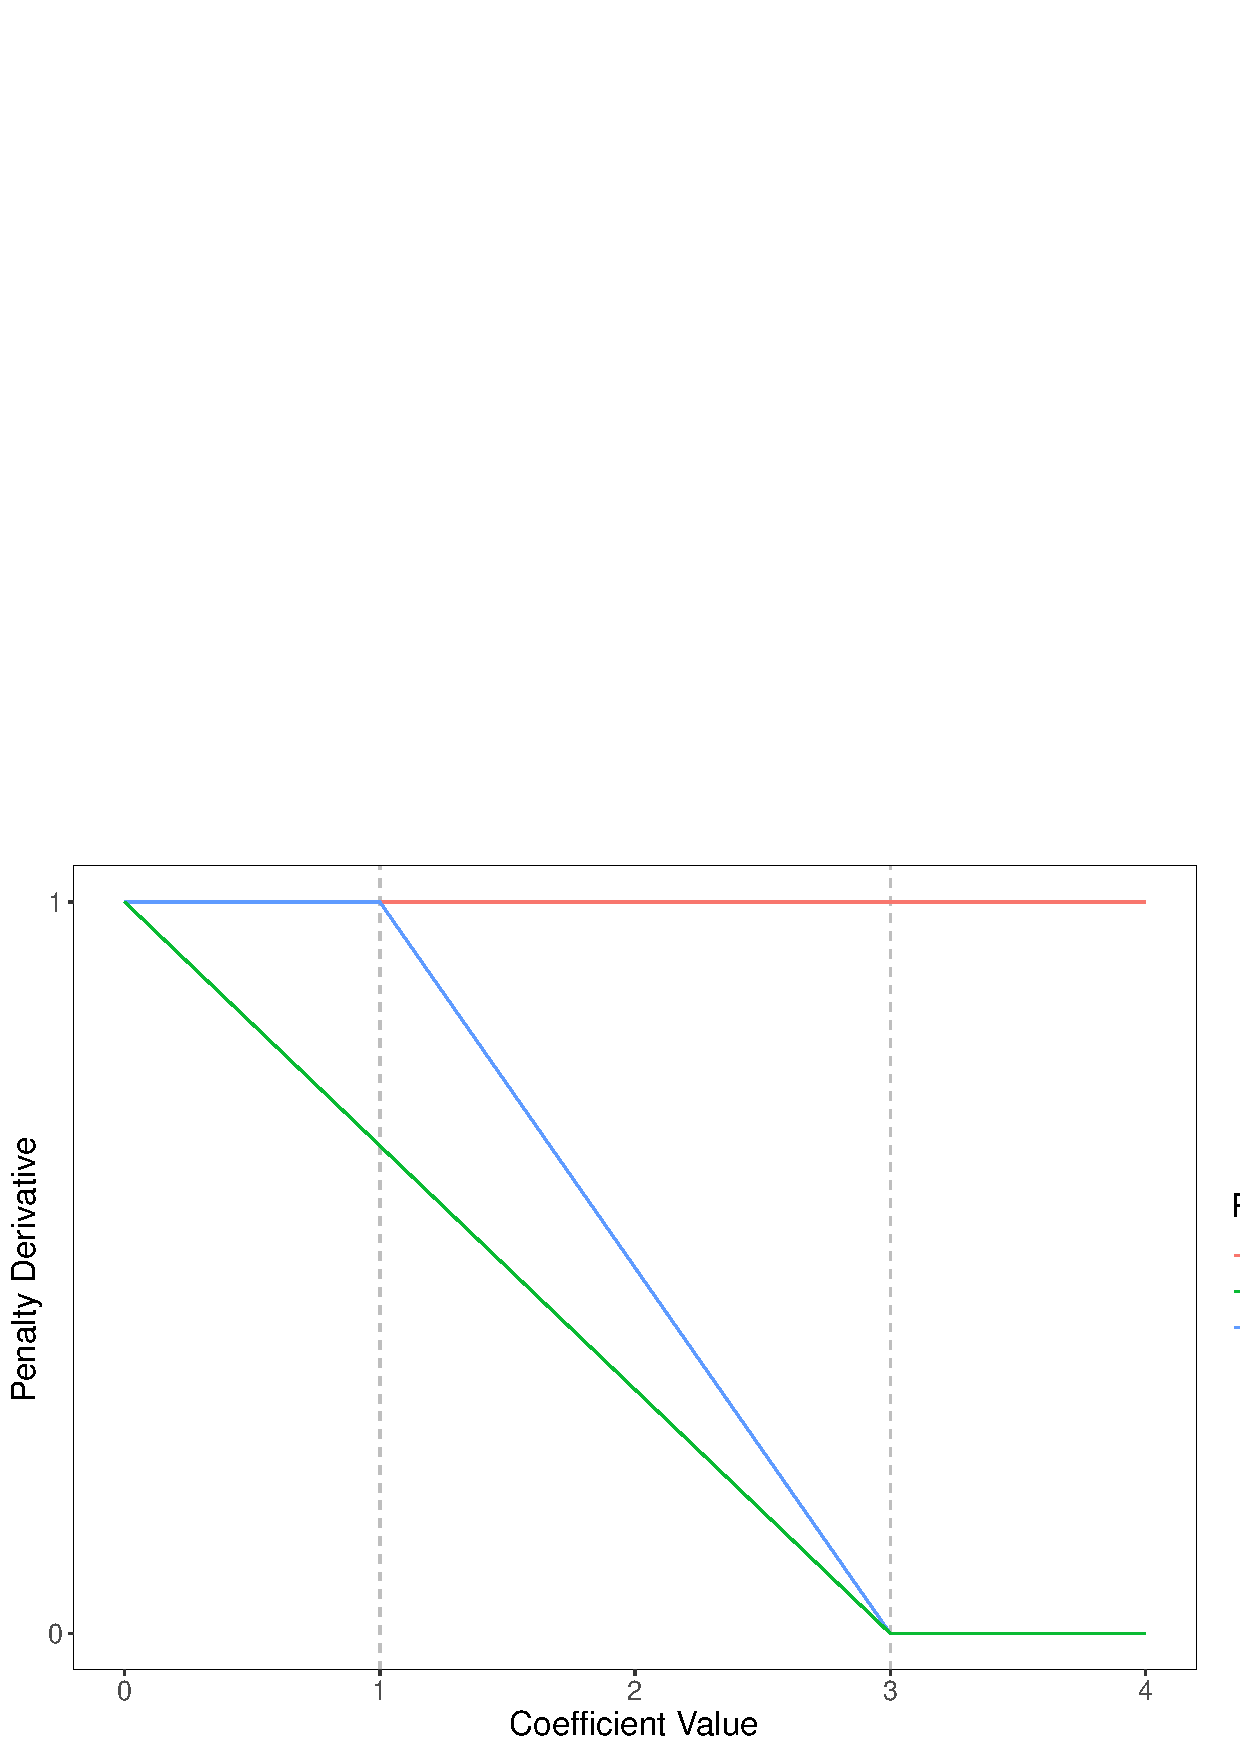
\includegraphics[width=\textwidth]{images/lasso-scad-mcp-derivative.png}
		\captionsetup{width = 0.8\textwidth}
		\caption{Derivatives of the penalty functions for lasso, SCAD, and MCP.}
		\label{fig:derivative}
	\end{subfigure}
	\captionsetup{width = 0.9\textwidth}
	\caption{Penalty functions for lasso, SCAD, and MCP, as well as their derivatives. These plots use $\lambda = 1$ and $a = 3$. The dashed vertical lines are the knots for SCAD and MCP.}
	\label{fig:lasso-scad-mcp}
\end{figure}

Note that of the penalized regression methods discussed above, only ridge regression has a general closed-form solution. Although lasso, elastic-net, SCAD and MCP do not have closed-form solutions, their solutions can be efficiently approximated \cite{friedman2010regularization, breheny2011ncvreg}. In some special cases, however, a closed-form solution exists. 

Let $\mathbf{X}$ be a $n\times p$ matrix where each row contains the predictor values for one observation. To simplify things, we will assume that our data is centralized so that the coefficient $\beta_0$ is 0; that way, we do not need to include an extra entry of 1 in each row of $\mathbf{X}$. In an \textbf{orthonormal design}, we assume that $\mathbf{X}$ is orthonormal, meaning that the magnitude of each column of $\mathbf{X}$ is one and every pair of columns of $\mathbf{X}$ is orthogonal. In this special case, the matrix $(\mathbf{X}^\top \mathbf{X})^{-1}$ is the $p\times p$ identity matrix. As a result, each coefficient is independent of the other coefficients; in other words, we can compute the coefficient estimate for each predictor without needing to use the values for the other predictors. For example, in an orthonormal design, the general solution to ordinary least squares regression given in Equation \ref{eqn:ols-solution} simplifies to
\begin{equation}\label{ols-orthonormal-solution}
	\hat{\bm{\beta}}^{\text{OLS}} = \mathbf{X}^\top \mathbf{y}
\end{equation}

To compute the coefficient estimates for lasso, SCAD, and MCP in an orthonormal design, we first compute the vector $\mathbf{z} = \mathbf{X}^\top \mathbf{y}$ \cite{fan2001variable}. Each entry of $\mathbf{z}$ corresponds to one predictor. We then apply a \textbf{thresholding function} to each entry of $\mathbf{z}$ to get the coefficient estimate for that predictor. For lasso, elastic-net, SCAD, and MCP, a closed-form for this thresholding function exists \cite{tibshirani1996regression, fan2001variable, zou2005regularization, zhang2010nearly}. The input to the thresholding function is the actual coefficient value, and the output is the estimated value for that coefficient in an orthonormal design. Figure \ref{fig:prediction} shows the threshold functions for lasso, SCAD and MCP when $\lambda = 1$. For SCAD and MCP, we used the value $a = 3$. For reference, the identity line is included, which can be considered as the threshold function for ordinary least squares.

\begin{figure}[!h]
	\centering
	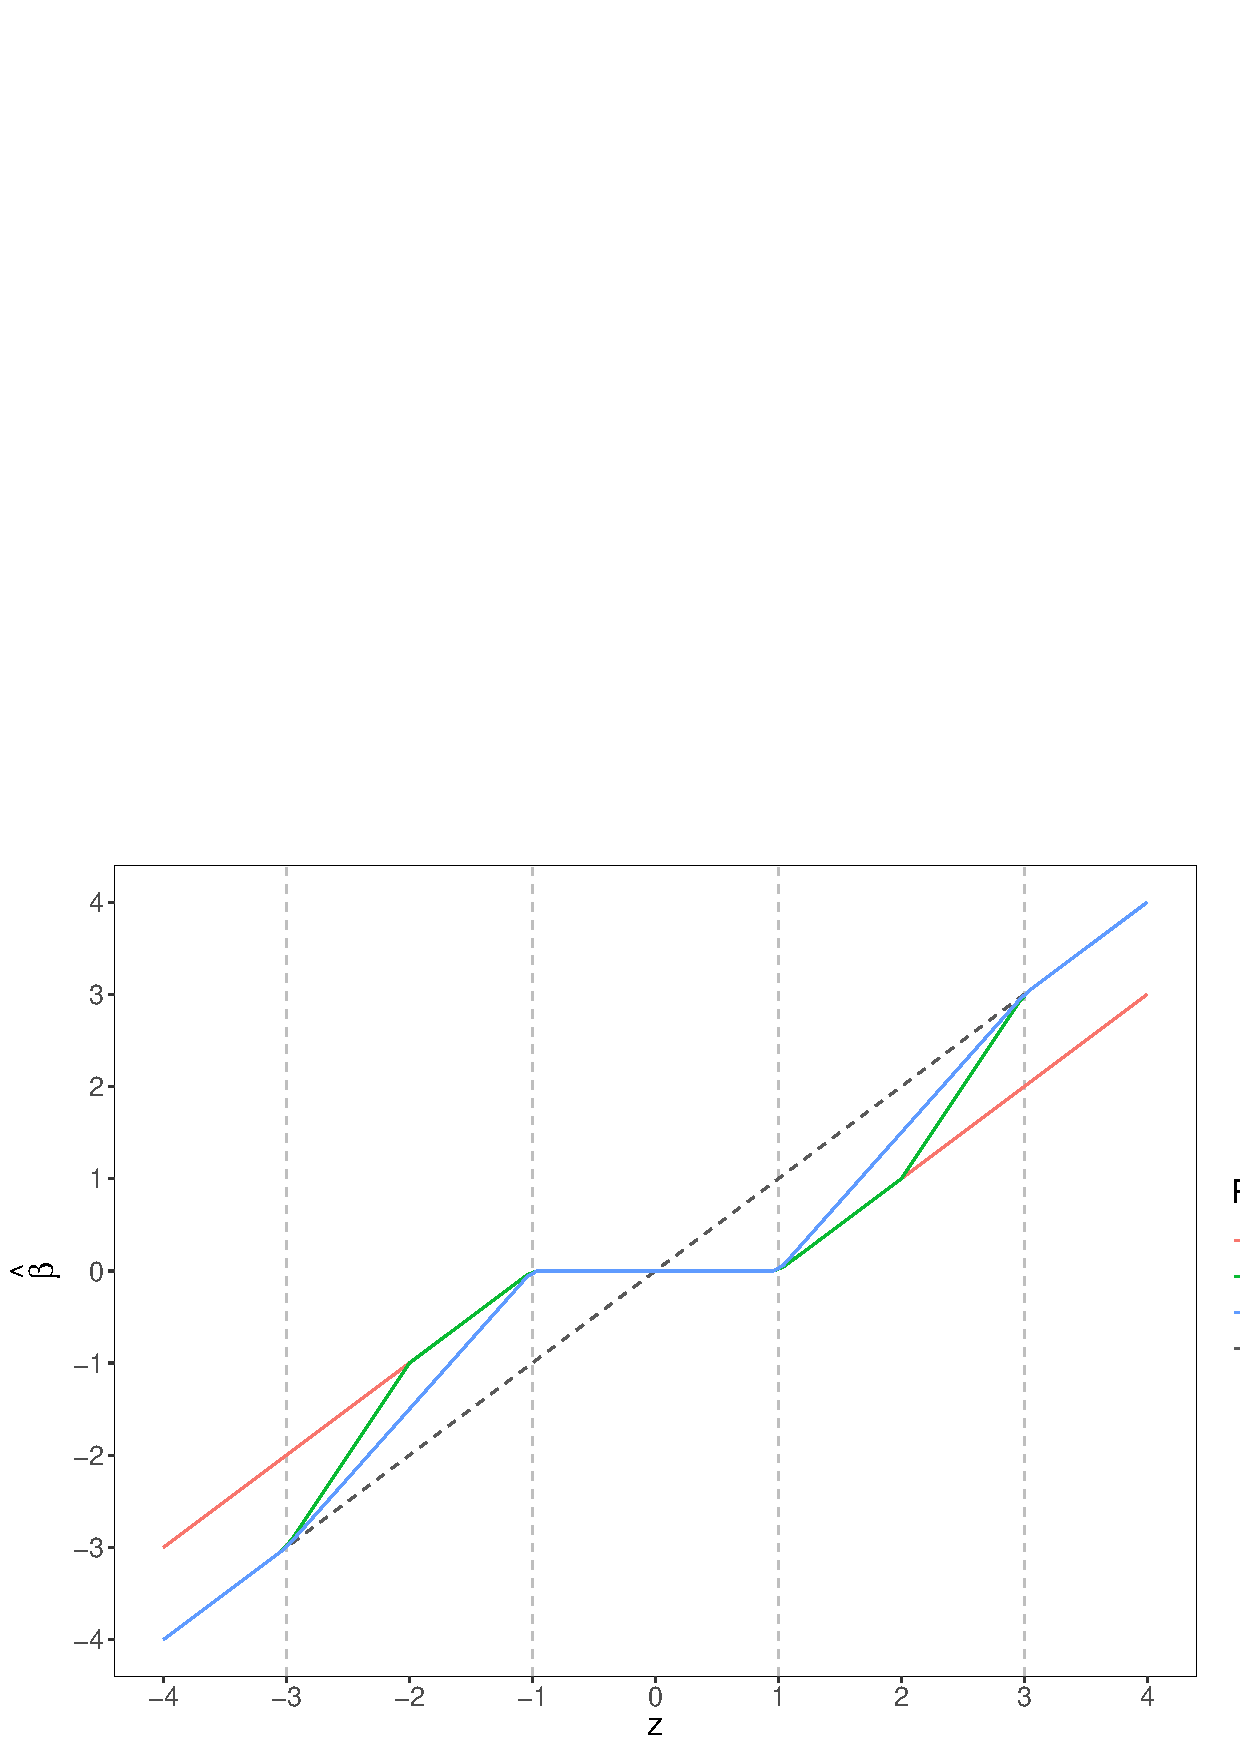
\includegraphics[width = 0.8\textwidth]{images/lasso-scad-mcp-solution.png}
	\captionsetup{width = 0.8\textwidth}
	\caption{Thresholding function for lasso, SCAD, and MCP when $\lambda = 1$ and $a = 3$ in an orthonormal design. The input ($z$) represents an entry from the vector $\mathbf{z}=\mathbf{X}^\top \mathbf{y}$; the output ($\hat{\beta}$) is the coefficient estimate. The dashed vertical lines are the knots for SCAD and MCP.}
	\label{fig:prediction}
\end{figure}

We see that when $\vert z \vert$ is small, the thresholding function for lasso, SCAD, and MCP are all zero. This matches with the assumption that these methods should set small coefficient estimates to zero. As $\vert z \vert$ increases, the estimated value for that coefficient gets larger. Notice that ordinary least squares doesn't decrease the estimated coefficient value for any choice of $z$; this is because of the fact that ordinary least squares is unbiased, whereas the other methods are biased.

In this figure, we also see that the threshold function for lasso is parallel to the identity line for large values of $\beta$. This means that even if a predictor is very influential on the response, lasso will predict a coefficient estimate that is less than the true coefficient value. This makes lasso a very biased model. This issue was one of the main motivations for SCAD and MCP. Unlike lasso, SCAD and MCP converge to the identity line as $\beta$ increases, which makes these methods less likely to decrease large coefficient estimates.

Another feature of SCAD and MCP is their oracle-like properties \cite{fan2001variable, zhang2010nearly}. The term \textbf{oracle} in this context was first proposed by Donohe and Johnstone in \cite{donoho1994ideal}. Suppose that a linear model could be fitted with the aid of an oracle. This oracle could tell you the subset of predictors that are truly related to the response so that a model can be fitted using only the important predictors. Although such a model is not possible in practice, this oracle procedure serves an ideal that can be worked towards.

\subsection{Non-linear models}
We next discuss several non-linear methods for regression: random forests, gradient boosting, and support vector machines.

\textbf{Random Forest} models (RF) are tree-based and solve the issue of high variance from individual decision trees by aggregating the predictions of many independent decision trees \cite{breiman2001random}. Each tree is fit using a subset of the observations and a subset of the predictors so that the trees are relatively independent from one another.

To fit each decision tree within a random forest model, we first select a random sample of the $n$ observations with replacement, in a process called \textbf{bootstrapping} \cite{efron1994introduction}. The number of observations chosen for each tree is a hyperparameter that can be changed. After selecting a set of observations, a random sample of predictors are chosen out of the $p$ predictors without replacement. Again, this helps decorrelate the trees. The number of predictors used in each tree is also a hyperparameter that can be changed. A decision tree is then generated using the available observations and predictors.

A random forest model aggregates all of the individual decision trees into a single model. The number of trees generated, $B$, is a hyperparameter that can be changed; usually, a random forest model will contain at least several hundred trees. To make predictions with a random forest, a test observation is passed into each decision tree and the predictions from each tree are aggregated. Figure \ref{fig:random-forest} demonstrates how a prediction is made using a random forest. For regression, the results are normally aggregated using the mean; for classification, the prediction chosen most often by the trees is usually used as the final prediction. 

\begin{figure}[h!]
	\footnotesize
	\centering
	\begin{forest}
	[Test observation,inner sep = 0.2cm, rounded corners, minimum height = 0.6cm, draw = black, fill = cyan!20
		%Tree 1
		[,circle,draw,fill=cyan,edge={->},label=Tree 1
			[,circle,draw,fill=cyan
				[,circle,draw
					[,circle,draw]
					[,circle,draw]
				]
				[,circle,draw,fill=cyan
					[,circle,draw]
					[,circle,draw,fill=cyan
						[Prediction 1,edge={->},inner sep = 0.2cm, rounded corners, minimum height = 0.6cm, draw = black, fill = green!20] {
							\draw[->] () to (agg);
						}
					]
				]
			]
			[,circle,draw
				[,circle,draw
					[,circle,draw]
					[,circle,draw]
			]
				[,circle,draw
					[,circle,draw]
					[,circle,draw]
				]
			]
		]
		% Tree 2
		[,circle,draw,fill=cyan,edge={->},label={[xshift=-2em,font=\small]Tree 2}
			[,circle,draw
				[,circle,draw
					[,circle,draw]
					[,circle,draw]
				]
				[,circle,draw
					[,circle,draw]
					[,circle,draw]
				]
			]
			[,circle,draw,fill=cyan
				[,circle,draw,fill=cyan
					[,circle,draw]
					[,circle,draw,fill=cyan
						[Prediction 2,edge={->},inner sep = 0.2cm, rounded corners, minimum height = 0.6cm, draw = black, fill = green!20
							[Aggregate result,edge={->},inner sep = 0.2cm, rounded corners, minimum height = 0.6cm, draw = black, fill = cyan!20,name=agg]
						]
					]
				]
				[,circle,draw
					[,circle,draw]
					[,circle,draw]
				]
			]
		]
		[..., l*=2,edge={->},inner sep = 0.2cm, rounded corners, minimum height = 0.6cm, draw = black, fill = cyan!20
			[...,l*=3,edge={->},inner sep = 0.2cm, rounded corners, minimum height = 0.6cm, draw = black, fill = green!20] {
			\draw[->] () to (agg);
			}
		]
		% Tree 3
		[,circle,draw,fill=cyan,edge={->},label=Tree $B$
			[,circle,draw
				[,circle,draw
					[,circle,draw]
					[,circle,draw]
				]
				[,circle,draw
					[,circle,draw]
					[,circle,draw]
				]
			]
			[,circle,draw,fill=cyan
				[,circle,draw
					[,circle,draw]
					[,circle,draw]
				]
				[,circle,draw,fill=cyan
					[,circle,draw]
					[,circle,draw,fill=cyan
						[Prediction $B$,edge={->},inner sep = 0.2cm, rounded corners, minimum height = 0.6cm, draw = black, fill = green!20] {
							\draw[->] () to (agg);
						}
					]
				]
			]
		]
	]
\end{forest}
	\captionsetup{width = 0.8\textwidth}
	\caption{Visualization of how predictions are made using a random forest model. An observation is input into each decision tree. Predictions from each tree are then aggregated into a single result that is used as the final prediction.}
	\label{fig:random-forest}
\end{figure}

This idea of fitting multiple models with bootstrapping and aggregating the results can be used with other models besides decision trees. In general, this process is called \textbf{bagging} (a combination of the words ``bootstrap'' and ``aggregating'') \cite{breiman1996bagging}. 

\textbf{Boosting} is the technique of sequentially improving a weak learner until it becomes a strong learner \cite{schapire1990strength}. A \textbf{gradient boosting machine} (GBM) is a boosting technique that uses gradient descent to minimize error in a model and correct the shortcomings of the previous model \cite{friedman2001greedy}. Boosting can be used on different types of models, but decision trees are the most common to use. Unlike random forest models, where each tree is independent of one another, the trees in a boosting model are grown sequentially. Each tree is fitted to correct the mistakes made by the previous tree. The details of how errors are corrected depends on the algorithm selected. With regression, each tree can be fitted by using the residuals from the previous tree as the training data \cite{james2013introduction}. Like random forest models, predictions are made by aggregating the results from each individual tree. See figure \ref{fig:boosting} for a diagram of how a boosting model is fitted.

\begin{figure}[b!]
	\footnotesize
	\centering
	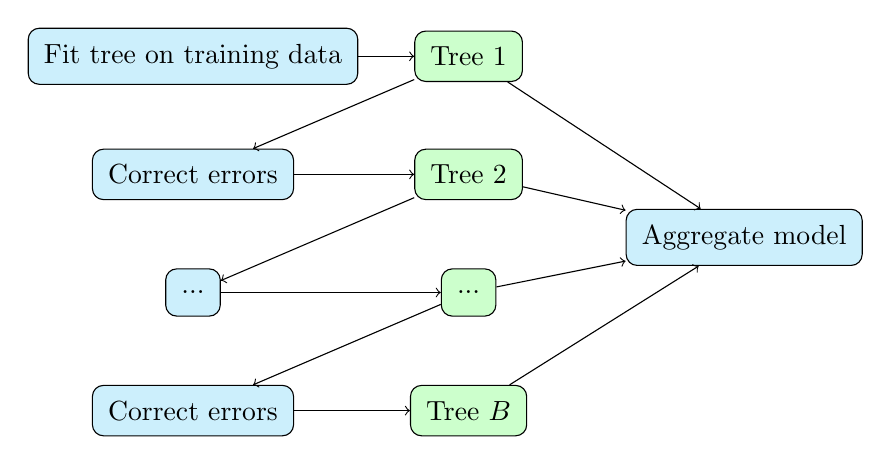
\begin{tikzpicture}
	\node (fit1)[fit]{Fit tree on training data};
	\node (tree1)[tree, right of = fit1, xshift = 2.5cm]{Tree 1};
	\node (fit2)[fit, below of = fit1, yshift = -0.5cm]{Correct errors};
	\node (tree2)[tree, right of = fit2, xshift = 2.5cm]{Tree 2};
	\node (fit3)[fit, below of = fit2, yshift = -0.5cm]{...};
	\node (tree3)[tree, right of = fit3, xshift = 2.5cm]{...};
	\node (fit4)[fit, below of = fit3, yshift = -0.5cm]{Correct errors};
	\node (tree4)[tree, right of = fit4, xshift = 2.5cm]{Tree $B$};
	\node (end)[fit, right of = tree2, xshift = 2.5cm, yshift = -0.8cm]{Aggregate model};
	
	\draw [->] (fit1) -- (tree1);
	\draw [->] (tree1) -- (fit2);
	\draw [->] (fit2) -- (tree2);
	\draw [->] (tree2) -- (fit3);
	\draw [->] (fit3) -- (tree3);
	\draw [->] (tree3) -- (fit4);
	\draw [->] (fit4) -- (tree4);
	
	\draw [->] (tree1) -- (end);
	\draw [->] (tree2) -- (end);
	\draw [->] (tree3) -- (end);
	\draw [->] (tree4) -- (end);
\end{tikzpicture}
	\captionsetup{width = 0.8\textwidth}
	\caption{How a boosting model with decision trees is fitted. Each tree is fitted to correct the errors of the previous tree. Predictions are made by combining the results from each decision tree.}
	\label{fig:boosting}
\end{figure}

Gradient boosting machines that use decision trees can be used for both regression and classification. When using a gradient boosting model with decision trees, \textbf{relative variable importance} and \textbf{pruning} can be used as a sort of pseudo-variable selection method to lower complexity and prevent over-fitting. However, this does not yield the same interpretability or bias trade off benefits that true variable selection yields./

Gradient boosting models often suffer from slow computation speeds due to the large number of sequential models that need to be trained. \textbf{Extreme Gradient Boosting} (XGBoost) is a faster version of gradient boosting that utilizes parallel computing as well as different optimization techniques to speed up computation \cite{chen2016xgboost}. For these reasons, XGBoost is often preferred over standard gradient boosting models and is very commonly used in many machine learning applications. In this study, we will use the XGBoost algorithm for gradient boosting.

There are a few different hyperparameters that can control how an XGBoost model is fit. The learning rate controls how quickly the gradient boosting model learns. If this learning rate is high, then the model learns quickly, but it may not learn as efficiently. If the learning rate is low, then the model takes longer but typically makes better predictions. The maximum tree depth determines how high each tree can be. Using smaller tree sizes may oversimplify the model, but it could also mitigate overfitting.

The final non-linear model that we considered is the \textbf{support vector machine} (SVM) \cite{cortes1995support}. Support vector machines are versatile models that can be used for both classification and regression. Originally, a support vector machine was designed as a binary classifier that separates the two response classes with a hyperplane in $(p - 1)$-dimensional space. The hyperplane chosen by a support vector machine is chosen to maximize the distance between the hyperplane and any of the observation points. The observations closest to this separating hyperplane are called \textbf{support vectors}. Predictions are made by determining which side of the hyperplane an observation lies on. Observations that lie above the hyperplane are assigned to one class, and observations on the other side are predicted to be the other class. Figure \ref{fig:svm} demonstrates a simple support vector machine for classification.

\begin{figure}[h!]
	\centering
	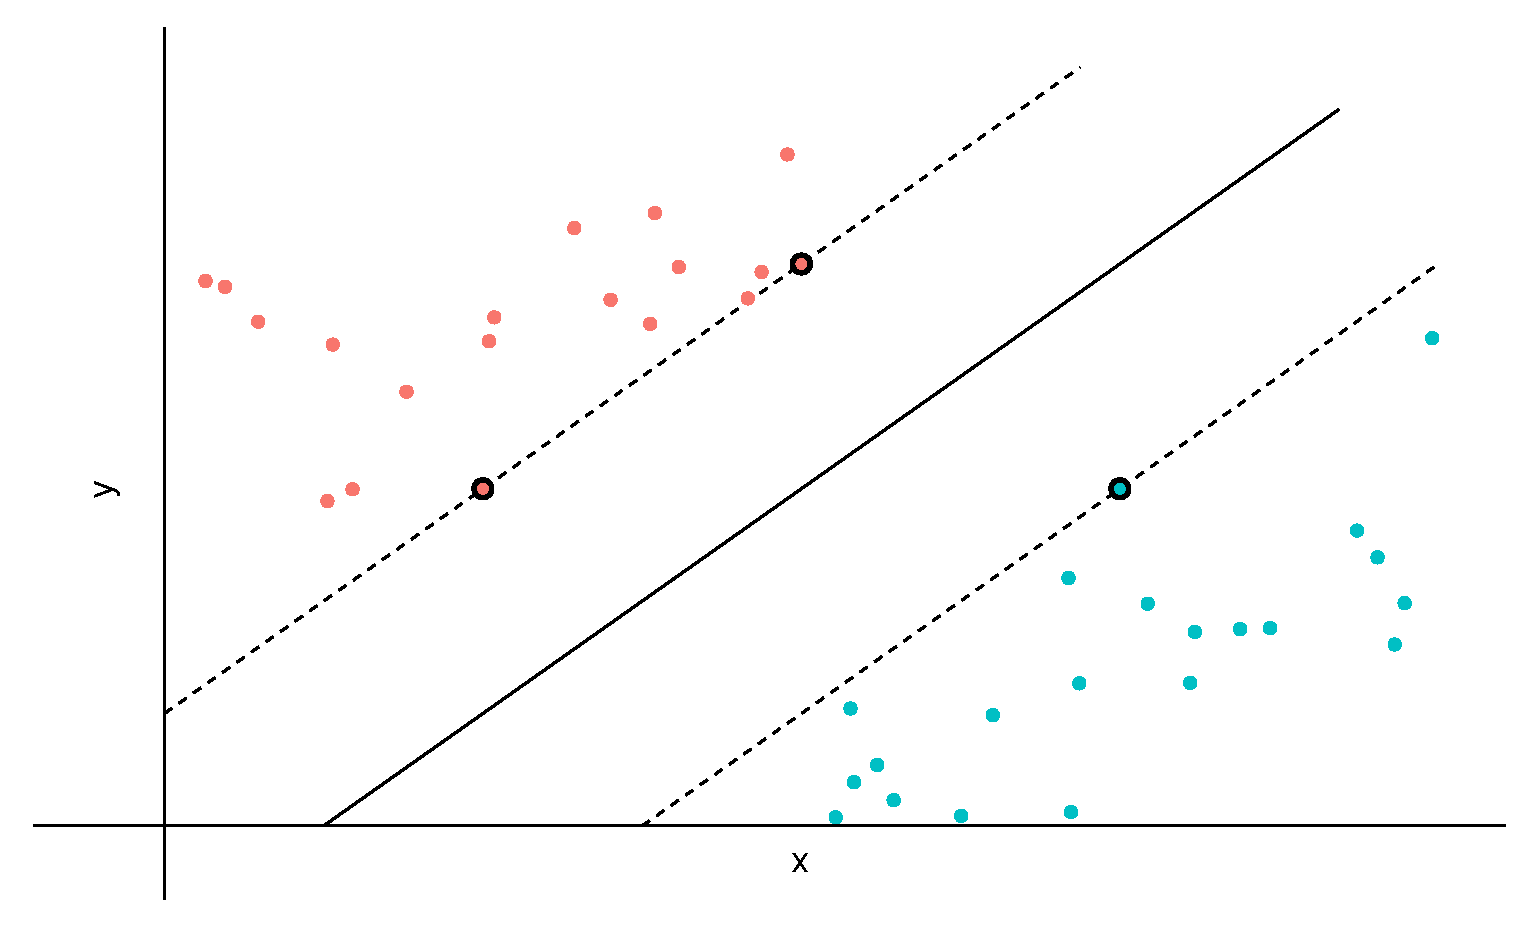
\includegraphics[width = 0.8\textwidth]{images/svm.eps}
	\captionsetup{width = 0.8\textwidth}
	\caption{Visualization of a simple support vector machine for binary classification. The solid black line is the hyperplane that maximizes the margin between the two classes. The points with a black outline are the support vectors. They are the points that define the hyperplane.}
	\label{fig:svm}
\end{figure}

Note that in most data sets, the classes cannot be split perfectly into two sides. Furthermore, this model has very high variance as changing the points near the hyperplane can significantly alter the hyperplane. Finally, this model cannot handle cases where the true boundary is non-linear. Luckily, support vector machines in practice can handle such issues. Typically, support vector machines are allowed to misclassify some of the training data, which address the cases where the data cannot be split perfectly by a hyperplane. Also, the predictor space can be enlarged to handle non-linear decision boundaries; this is typically done by using \textbf{kernels}. For example, using a radial kernel can create decision boundaries that enclose regions of the $p$-dimensional space.

Support vector machines can also be generalized to handle classification when there are more than two classes. They can also be used for regression \cite{drucker1997support}. We will be using support vector machines for regression in our study.

Like the other non-linear methods, there are many different hyperparameters that can be tuned. The two hyperparameters that we considered are $\epsilon$ and the cost function. The hyperparameter $\epsilon$ defines how tolerant the algorithm is of small errors. If $\epsilon$ is large, then the support vector machine will tolerate larger errors; if $\epsilon$ is small, then even small errors will be punished. The cost hyperparameter $C$ determines how strongly the model punishes incorrect predictions. If $C$ is large, then the model punishes incorrect predictions more, making it fit more tightly to the training set. If $C$ is smaller, then the model is likely to allow more incorrect predictions in the training data.

\newpage
\bibliographystyle{plain-lf}
\bibliography{references}
\end{document}